\documentclass[11pt]{article}

\usepackage[margin=0.85in]{geometry}
\usepackage[utf8]{inputenc}
\usepackage[T1]{fontenc}
\usepackage{lmodern}
\usepackage{graphicx}
\usepackage{booktabs}
\usepackage{array}
\usepackage{xcolor}
\usepackage{hyperref}
\usepackage{enumitem}

\hypersetup{
  colorlinks=true,
  linkcolor=blue!45!black,
  urlcolor=blue!45!black
}

\setlength{\parindent}{0pt}
\setlength{\parskip}{0.55em}
\renewcommand{\arraystretch}{1.18}
\renewcommand{\figurename}{Figura}
\renewcommand{\tablename}{Tabla}

\title{\textbf{Variables de decisión para el paper SCRES-RL de Garrido}\\
\large Nota de reunión: Track B, control post-CDC, buffers y KAN/CAN}
\author{Preparado para discusión con el Prof. Garrido y David}
\date{3 de julio de 2026}

\begin{document}
\maketitle

\section*{Propósito}

Esta nota separa dos decisiones que quedaron mezcladas en la reunión:

\begin{enumerate}[leftmargin=1.5em]
  \item \textbf{Superficie de decisión:} qué variables de la cadena de suministro puede controlar el agente.
  \item \textbf{Arquitectura neuronal:} si el controlador será PPO+MLP, PPO recurrente, DMLPA/CAN o KAN.
\end{enumerate}

La evidencia actual indica que estas decisiones deben tomarse en ese orden.
Primero se debe congelar una superficie de decisión físicamente defendible.
Luego se corre la arquitectura neuronal sobre esa superficie. Una red más
potente no puede rescatar una superficie de decisión que viola conservación de
inventario o que no alcanza el cuello de botella operacional.

\section*{Recomendación para la reunión}

\textbf{Ruta recomendada para Paper 1:} mantener la superficie de decisión
probada de Track B como línea principal del paper. Tiene la evidencia más
fuerte, no crea inventario y responde la pregunta central: RL mejora SCRES
cuando el espacio de acción llega al cuello de botella de recuperación aguas
abajo.

\textbf{Extensión recomendada para Garrido:} si el Prof. Garrido quiere buffers
literales post-CDC, implementarlos como un \emph{sidecar conservador}: se
permiten objetivos continuos de buffer, pero la reposición debe ser un evento
DES limitado por inventario aguas arriba, capacidad, lead time y costo. Primero
se corre un gate estático/oráculo; sólo se entrena CAN/KAN si ese gate muestra
headroom real.

\textbf{Declaración sobre arquitectura:} KAN/CAN merece una oportunidad real.
Real-KAN ya mejora el ReT de Excel sobre PPO+MLP en 10/10 semillas pareadas,
pero con un costo de utilización mucho mayor. Esto lo convierte en un sidecar
arquitectónico fuerte y en una respuesta directa a la preocupación de Garrido
sobre KAN, pero todavía no reemplaza la columna vertebral PPO+MLP del paper.

\section*{Operaciones seleccionadas y criterio}

Las operaciones seleccionadas siguen la topología de la tesis y el límite
discutido en reunión: ``desde el Centro de Distribucion hacia abajo''. Op3 es
el CDC/WDC. La variante estricta post-CDC congela Op3 y deja sólo autoridad
aguas abajo.

\begin{figure}[ht]
  \centering
  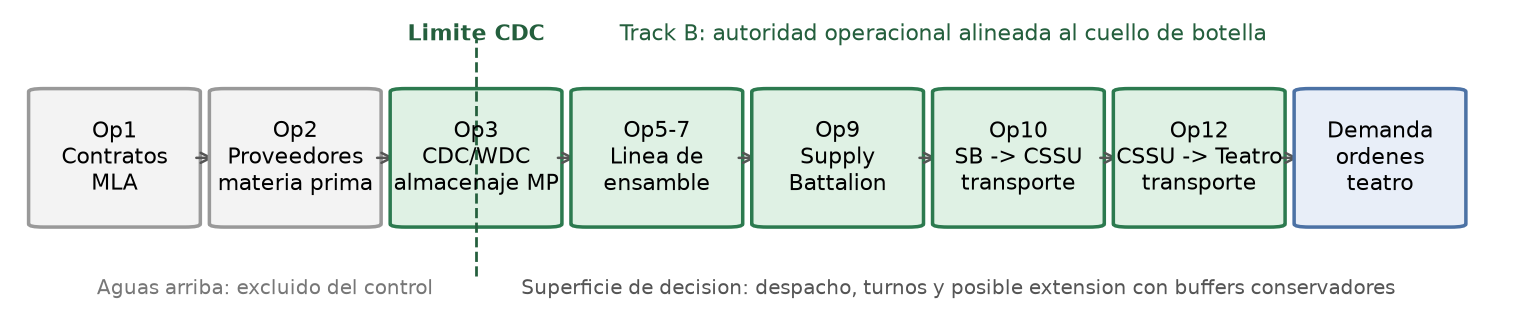
\includegraphics[width=\linewidth]{figures/fig1_topology_selected_operations_es.pdf}
  \caption{Operaciones seleccionadas en la topología de cadena de suministro basada en Garrido.}
\end{figure}

\begin{table}[ht]
\centering
\small
\begin{tabular}{p{0.12\linewidth}p{0.26\linewidth}p{0.27\linewidth}p{0.25\linewidth}}
\toprule
\textbf{Operación} & \textbf{Rol en la tesis} & \textbf{Criterio de selección} & \textbf{Variable de decisión} \\
\midrule
Op3 / CDC-WDC & Recibe, verifica y almacena materias primas. & Es el límite de reunión: ``CDC hacia abajo''. También permite probar si la autoridad sobre el CDC es necesaria. & En Track B completo: cantidad de despacho de materia prima y punto de reorden. En post-CDC estricto: congelada. \\
Op5-7 / Ensamble & Convierte materias primas en raciones. & Determina la capacidad de recuperación cuando se acumula demanda/backlog. & Nivel de turno, implementado como acción continua y mapeado a umbrales S1/S2/S3. \\
Op9 / Supply Battalion & Almacena y despacha raciones terminadas aguas abajo. & Primer buffer y punto de despacho de raciones aguas abajo. & Controles de cantidad/punto de reorden; nodo candidato para buffer conservador. \\
Op10 / SB a CSSU & Tramo de transporte desde Supply Battalion hacia CSSU. & Uno de los cuellos de botella de recuperación aguas abajo encontrados empíricamente. & Multiplicador de despacho para q-min/q-max. \\
Op12 / CSSU a Teatro & Tramo final de transporte hacia la demanda en teatro. & Segundo cuello de botella aguas abajo; afecta directamente las colas de recuperación de órdenes. & Multiplicador de despacho para q-min/q-max. \\
\bottomrule
\end{tabular}
\caption{Nodos de decisión seleccionados desde la topología de la tesis.}
\end{table}

\section*{Alternativa 1: control operacional de Track B}

Esta es la línea actualmente probada. No controla contratos de proveedores ni
procurement aguas arriba. Controla despacho CDC/aguas abajo y capacidad de
ensamble, con todos los movimientos de material restringidos por inventario
real.

\subsection*{Variables completas de Track B}

\begin{table}[ht]
\centering
\small
\begin{tabular}{p{0.18\linewidth}p{0.22\linewidth}p{0.48\linewidth}}
\toprule
\textbf{Variable} & \textbf{Nodo} & \textbf{Significado} \\
\midrule
\texttt{op3\_q} & Op3 / CDC & Cantidad semanal de despacho de materia prima desde CDC/WDC hacia ensamble. \\
\texttt{op3\_rop} & Op3 / CDC & Timing de reorden/despacho en el límite del CDC. \\
\texttt{op9\_q} & Op9 & Cantidad de despacho desde Supply Battalion. \\
\texttt{op9\_rop} & Op9 & Timing de despacho desde Supply Battalion. \\
\texttt{op5\_q} & Op5 & Presente en el contrato histórico, pero actualmente inerte salvo que se inicialice explícitamente un buffer Op5; no sostiene el resultado de Track B. \\
\texttt{shift} & Ensamble & Accion continua mapeada a turnos de ensamble S1/S2/S3. \\
\texttt{op10\_q} & Op10 & Multiplicador de despacho para el tramo SB-CSSU. \\
\texttt{op12\_q} & Op12 & Multiplicador de despacho para el tramo CSSU-teatro. \\
\bottomrule
\end{tabular}
\caption{Superficie de acción completa de Track B.}
\end{table}

\subsection*{Variante estricta post-CDC}

La variante estricta congela los controles de Op3/CDC en el baseline de Garrido
y mantiene sólo despacho aguas abajo más autoridad sobre turnos. Esto responde
directamente la pregunta: ¿depende el resultado de controlar el CDC? La respuesta es no.

\begin{itemize}[leftmargin=1.5em]
  \item ReT Excel de PPO post-CDC-only: 0.005838.
  \item Mejor comparador estático ReT Excel: 0.005428.
  \item Delta ReT a nivel de orden: +0.0003967.
  \item Signos por semilla: 5/5 positivos; signos por episodio pareado: 60/60 positivos.
\end{itemize}

\section*{Alternativa 2: buffers conservadores post-CDC}

Esta es la versión literal de la solicitud del Prof. Garrido: permitir buffers
en nodos después del CDC. La regla central es que el buffer no puede llenarse
por magia. Una acción continua es compatible con DES, pero la conservación de
inventario no es opcional.

\begin{figure}[ht]
  \centering
  \scriptsize
  \setlength{\fboxsep}{3pt}
  \makebox[\linewidth][c]{%
  \fbox{\parbox[c][0.62cm][c]{0.105\linewidth}{\centering Inventario\\aguas arriba}}
  \hspace{0.01\linewidth}$\rightarrow$\hspace{0.01\linewidth}
  \fbox{\parbox[c][0.62cm][c]{0.105\linewidth}{\centering Objetivo\\de decisión}}
  \hspace{0.01\linewidth}$\rightarrow$\hspace{0.01\linewidth}
  \fbox{\parbox[c][0.62cm][c]{0.12\linewidth}{\centering Evento DES\\orden/despacho}}
  \hspace{0.01\linewidth}$\rightarrow$\hspace{0.01\linewidth}
  \fbox{\parbox[c][0.62cm][c]{0.105\linewidth}{\centering Lead time\\+ capacidad}}
  \hspace{0.01\linewidth}$\rightarrow$\hspace{0.01\linewidth}
  \fbox{\parbox[c][0.62cm][c]{0.105\linewidth}{\centering Buffer\\aguas abajo}}%
  }

  \vspace{0.5em}
  \textcolor{green!45!black}{Regla de conservación: cantidad movida =
  $\min(\mathrm{faltante},\ \mathrm{disponible\ aguas\ arriba},\ \mathrm{capacidad})$.}

  \textcolor{green!45!black}{No hay top-up instantáneo; el agente no crea inventario.}
  \caption{Mecanismo físicamente conservador de reposición de buffers.}
\end{figure}

El mecanismo propuesto para buffers es:

\begin{enumerate}[leftmargin=1.5em]
  \item El agente elige un objetivo continuo de buffer para un nodo post-CDC.
  \item El DES agenda un evento de reposición/despacho.
  \item La cantidad enviada se limita por inventario aguas arriba y capacidad:
  \[
    q_{\mathrm{movida}} =
    \min(\mathrm{faltante},\ \mathrm{disponible\ aguas\ arriba},\ \mathrm{capacidad}).
  \]
  \item El material llega sólo después del lead time de proceso/transporte.
  \item Se registran costos de inventario, turnos y despacho.
\end{enumerate}

Esto no contradice la simulación de eventos discretos. DES significa que los
cambios de estádo del sistema ocurren mediante eventos; no exige que todas las
variables de decisión sean discretas. Los objetivos continuos son válidos
siempre que se materialicen mediante eventos discretos y restricciones de
conservación.

\subsection*{Cómo probar está alternativa}

No se debe entrenar PPO/CAN/KAN primero. Primero conviene correr un gate
estático/oráculo barato:

\begin{itemize}[leftmargin=1.5em]
  \item Congelar \texttt{op10\_q} y \texttt{op12\_q} en el ajuste probado de
  despacho aguas abajo de Track B, para no confundir ganancias de buffer con
  ganancias de despacho.
  \item Variar sólo objetivos de buffer en nodos post-CDC seleccionados: Op9,
  inventario CSSU después de Op10 e inventario de teatro después de Op12.
  \item Comparar el mejor oráculo condicionado por régimen contra la mejor
  política estática única de buffers, usando números aleatorios comunes.
  \item Entrenar CAN/KAN sólo si el gate de oráculo muestra headroom
  significativo más alla de la evidencia actual de Track B.
\end{itemize}

\section*{Resultados disponibles}

\begin{figure}[ht]
  \centering
  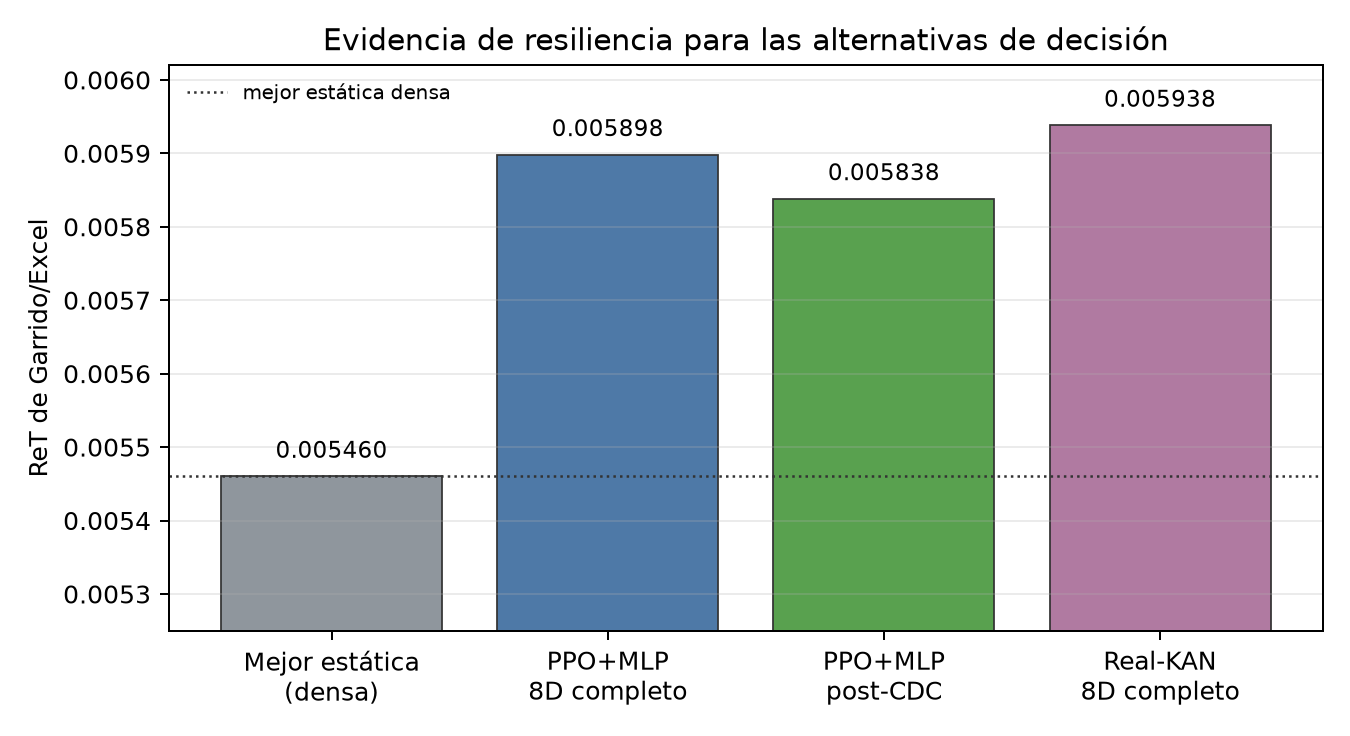
\includegraphics[width=0.82\linewidth]{figures/fig2_results_ret_bars_es.pdf}
  \caption{ReT Excel para las principales líneas de evidencia.}
\end{figure}

\begin{figure}[ht]
  \centering
  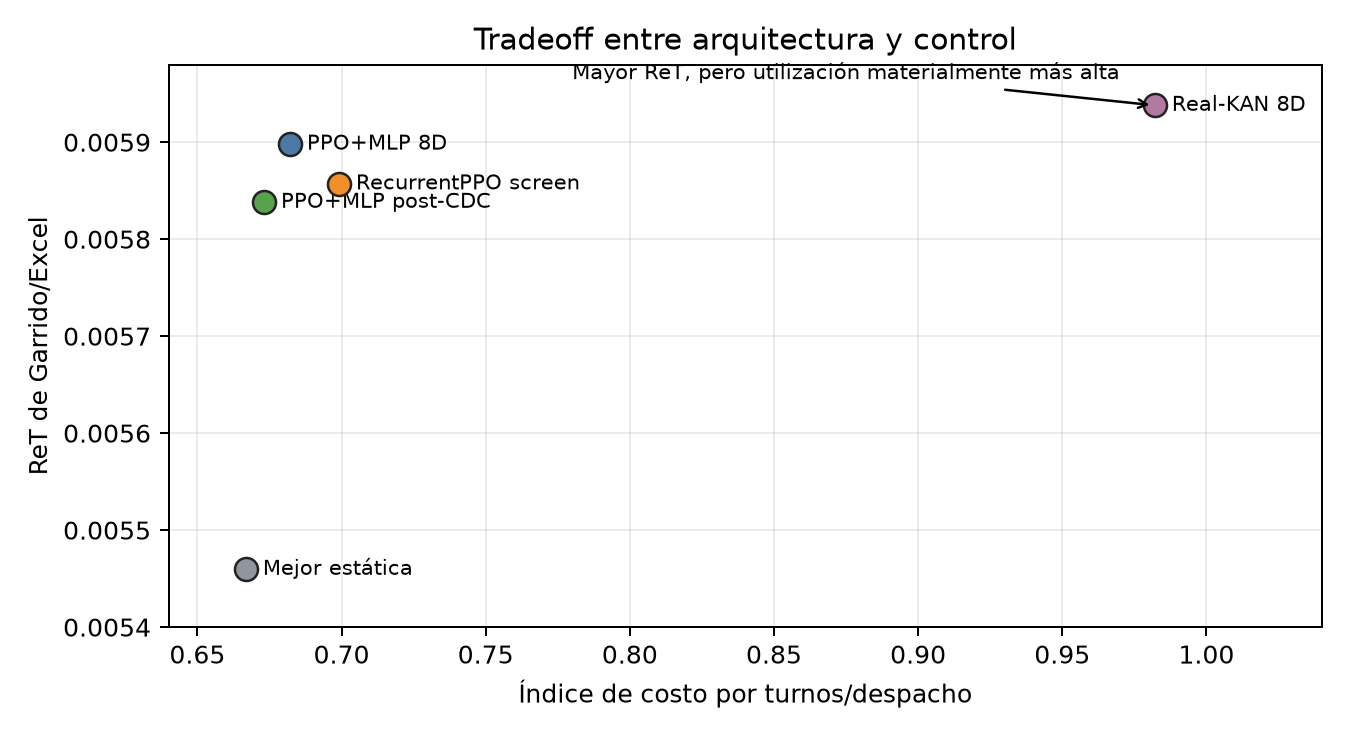
\includegraphics[width=0.82\linewidth]{figures/fig3_ret_cost_tradeoff_es.pdf}
  \caption{Tradeoff ReT-costo. Real-KAN mejora ReT, pero con mucha mayor utilización.}
\end{figure}

\begin{table}[ht]
\centering
\footnotesize
\begin{tabular}{p{0.30\linewidth}rrp{0.34\linewidth}}
\toprule
\textbf{Linea} & \textbf{ReT Excel} & \textbf{Delta} & \textbf{Interpretacion} \\
\midrule
Mejor estática densa & 0.005460 & -- & Baseline fuerte sin aprendizaje. \\
PPO+MLP Track B completo & 0.005898 & +0.000438 & Resultado principal de Paper 1; 10/10 semillas positivas vs estática. \\
PPO+MLP post-CDC estricto & 0.005838 & +0.000410 & No se requiere controlar el CDC; 5/5 semillas positivas. \\
RecurrentPPO/LSTM & 0.005857 & +0.000406 & La memoria sola supera a la estática, pero queda bajo PPO+MLP. \\
Real-KAN Track B completo & 0.005938 & +0.000041 & Mejor ReT vs PPO+MLP; 10/10 positivo, pero alto costo de utilización. \\
\bottomrule
\end{tabular}
\caption{Resumen de evidencia. La métrica primaria es ReT Garrido/Excel.}
\end{table}

\section*{Qué indica esto sobre capacidad de aprendizaje}

Ambas direcciones candidatas muestran capacidad de aprendizaje:

\begin{itemize}[leftmargin=1.5em]
  \item \textbf{Control operacional Track B} ya aprende: PPO+MLP supera
  estáticas densas, heuristicas, tablas de régimen, controles con observación
  enmascarada, y la variante post-CDC estricta sigue positiva.
  \item \textbf{Mejoras arquitectónicas} también aprenden en Track B:
  RecurrentPPO supera estáticas; DMLPA supera estáticas pero no supera PPO+MLP;
  Real-KAN supera PPO+MLP en ReT Excel en 10/10 semillas.
  \item \textbf{Control por objetivos de buffer} aún no está probado como línea
  de aprendizaje. Es defendible si se implementa conservadoramente, pero debe
  comenzar con un gate de oráculo antes de una corrida larga CAN/KAN.
\end{itemize}

\section*{Decisión solicitada al Prof. Garrido}

Proponemos dos rutas viables:

\begin{enumerate}[leftmargin=1.5em]
  \item \textbf{Ruta conservadora para Paper 1:} usar las variables de despacho
  operacional de Track B como paper principal, con PPO+MLP como aprendiz base
  limpio y Real-KAN como sidecar arquitectónico confirmado.
  \item \textbf{Ruta de buffers Garrido:} agregar objetivos conservadores de
  buffer post-CDC como sidecar. Si el gate estático/oráculo es positivo, correr
  un controlador CAN/KAN largo sobre esa superficie.
\end{enumerate}

Nuestra recomendacion es la ruta 1 para el envío Q1 porque ya está
estádísticamente soportada y es físicamente conservadora. La ruta 2 es la forma
correcta de responder la pregunta literal de buffers, pero no debería retrasar
el paper actual salvo que el Prof. Garrido prefiera ese enfasis científico.

La decisión final queda a disposición del Prof. Garrido. Podemos avanzar con la
superficie de decisión que considere más significativa para el paper, siempre
que el mecanismo de reposición siga siendo físicamente conservador y la métrica
primaria siga siendo la fórmula de resiliencia Excel de Garrido.

\end{document}
